%%%%%%%%%%%%%%%%%%%%%%%%%%%%%%%%%%%%%%%%%%%%%%%%%%%%%%%%%%%%%%%%%%%%%%%%%%%%%%%
% Chapter 3: Título del capítulo 3
%%%%%%%%%%%%%%%%%%%%%%%%%%%%%%%%%%%%%%%%%%%%%%%%%%%%%%%%%%%%%%%%%%%%%%%%%%%%%%%

\section{Tecnologías}
\label{3:sec1}

\subsection{Tecnologías populares}
\label{3:1:1}
{\bf Django - Python}
Django es un framework para aplicaciones web gratuito y open source, escrito en Python. Un conjunto de componentes que te ayudan a desarrollar sitios web más fácil y rápidamente siguiendo el patrón Modelo Vista Controlador.

{\bf Ruby on Rails - Ruby}
Ruby on Rails, también conocido como RoR o Rails, es un framework de aplicaciones web de código abierto escrito en el lenguaje de programación Ruby, siguiendo el patrón Modelo Vista Controlador (MVC).

{\bf Express.js - Javascript}
Espress.js  es un framework de desarrollo de aplicaciones web minimalista y flexible para Node.js. Está inspirado en Sinatra, además es robusto, rápido, flexible y muy simple, además, es compatible con el patrón Modelo Vista Controlador.

Aquí tenemos una pequeña comparación de la popularidad que han tenido estas tecnologías en el último año.

\subsection{Tecnologías Escogidas}
\label{3:1:2}

Finalmente se escogió Express.js, Node.js y Javascript como tecnologías principales a usar en este proyecto por las siguientes razones:

En primer lugar, el uso de Node.js como tecnología de servidor aporta una gran ventaja ya que Javascript se usa en ambos lados, en el backend y en el frontend, reduciendo complejidad y tiempo de desarrollo ya que Express es bastante fácil de aprender y usar. Además, JavaScript es el lenguaje de programación más popular en el desarrollo web.

\begin{figure}[!th]
\begin{center}
\includegraphics[scale=0.5]{images/comparativa}
\caption{Comparativa de Tecnologias usadas}
\label{fig:Comparativa de Tecnologias usadas}
\end{center}
\end{figure}

Además de eso, la comunidad de Node.js está en constante crecimiento: la cantidad de preguntas de StackOverflow aumenta constantemente, por lo que la base de conocimiento para la tecnología es amplia. También hay que destacar el hecho de que Node.js sea de código abierto y gratuito. 

Finalmente, Node nos ofrece NPM, un gestor de paquetes que dispone de una gran cantidad de paquetes que crece rápidamente y aporta una forma sencilla de gestionar los paquetes que necesitemos en nuestro proyecto.

{\bf NPM}

NPM es un administrador de paquetes para Node.js con cientos de miles de paquetes. Aunque crea parte de la estructura del directorio del proyecto, este no es el objetivo principal.

El objetivo principal, es la automatización de dependencias y gestión de paquetes de cada proyecto. Esto significa que puede especificar todas las dependencias de su proyecto dentro del fichero package.json usando el comando npm i -s nombrepaquete, de forma que cada vez que un usuario clone el proyecto en su máquina simplemente tenga ejecutar npm install e inmediatamente se descargan e instalan todas las dependencias necesarias para el funcionamiento del proyecto en el directorio node modules/. Además, también sirve para especificar en qué versión está su proyecto.

También es posible descargar manualmente los paquetes, copiarlo en el directorio nodemodules/ y usarlo de esa manera. Sin embargo, a medida que crezca el proyecto y la lista de dependencias, llevará mucho tiempo instalar los paquetes necesarios y será una tarea engorrosa. También hace que colaborar y compartir tu proyecto sea mucho más difícil

{\bf Express.js}

Express es un framework ‘’minimalista’’ que permite crear una infraestructura web simple sobre Node.js. Express permite crear una API REST, un tipo de arquitectura de desarrollo web que se apoya totalmente en el estándar HTTP:

\begin{itemize}
  \item GET: Para consultar y leer recursos
  \item POST: Para crear recursos
  \item PUT: Para editar recursos
  \item DELETE: Para eliminar recursos
  \item PATCH: Para editar partes concretas de un recurso
\end{itemize}

Express también permite crear una aplicación web siguiendo el patrón de diseño Modelo Vista Controlador, que separa los datos y la lógica de de una aplicación de su representación.

{\bf Github API}

Para poder usar Github como estructura necesitaremos hacer uso de su Github REST API v3. 
La API nos permitirá acceder a los servicios que ofrece Github de forma externa, es decir, podremos crear repositorios, usar organizaciones como clases y manejar otros servicios, como consulta de información sobre el usuario.
Para poder acceder a la clave de cada usuario, debemos usar un Token generado por Github, es decir, una cadena que nos permitirá  identificarnos para realizar transacciones usando la API, en este caso, el token será generado usando las aplicaciones OAuth que nos ofrece Github para que el usuario haga login con su cuenta de usuario de github, sin necesidad de poner su usuario y contraseña de Github en la plataforma Codelab.
La Github REST API v3 tiene además varias librerías de terceros y tres librerías oficiales escritas en Ruby, Javascript y .Net.

{\bf MongoDB}

MongoDB es un sistema gestor de base de datos NoSQL, es decir, MongoDB es un sistema de bases de datos no relacional, en lugar de almacenar los datos en tablas, se almacenan colecciones o documentos, que está formado por objetos, y estos a su vez por claves y cada clave tiene un valor asociado. Es decir, sería algo parecido a un documento JSON, aunque en MongoDB usan una distribución llamada BSON.

\begin{figure}[!th]
\begin{center}
\includegraphics[scale=0.5]{images/nosql}
\caption{NoSQL vs SQL}
\label{fig:NoSQL vs SQL}
\end{center}
\end{figure}

{\bf Mongoose}

Mongoose es un una herramienta para el diseño de objetos de MongoDB. 
Mongoose provee una serie de métodos y funciones para manejar la base de datos en MongoDB.

{\bf Motor de vistas}

Como motor de vistas para el proyecto se ha elegido Pug, antes conocido como Jade, un motor de vistas implementado en Javascript para su uso en NodeJS y que dispone de una fácil integración con Express.JS. 

{\bf Automatización de tareas}

Para la automatización de tareas como generar el fichero de variables de entorno o poner en marcha un servidor nodemon se ha usado Gulp, una herramienta que permite automatizar tareas en Node.js, es simple y bastante fácil de usar.

{\bf Framework de CSS}

Como framework para los estilos de CSS se ha usado Materialize CSS, basado en material design. Ofrece varias opciones a la hora de diseñar la plataforma, permitiendo un diseño más minimalista o un diseño más cargado y vistoso.

%++++++++++++++++++++++++++++++++++++++++++++++++++++++++++++++++++++++++++++++
\section{Github API}
\label{3:sec2}

Para poder usar Github como estructura para la creación de aulas y tareas de código usaremos la Github REST API V3.
La API permite acceder a las funcionalidades de Github, A continuación se detallará que funcionalidades de la Github API se han usado

\begin{itemize}
  \item Oauth
  \item Organizaciones, Repositorios y Equipos
\end{itemize}

\subsection{OAuth}
\label{3:2:1}

La funcionalidad más básica que se usa es OAuth, que permite loguear al ususario con su cuenta de Github en
Codelab.

OAuth, sigla de Open Authorization es un estándar de código abierto que permite a un usuario compartir su información de un proveedor de servicios, como Google, Twitter, Facebook o en este caso de Github, con un consumidor, en nuestro caso Codelab.

Desde el punto de vista de Codelab, OAuth proporciona un método de acceso a los datos de Github a la vez que se protegen los credenciales de la cuenta.

Desde Codelab, solicitamos al usuario una serie de accesos y permisos en sus datos, para poder operar con las organizaciones y repositorios de Github.

\begin{figure}[!th]
\begin{center}
\includegraphics[scale=0.5]{images/permisos}
\caption{Vista de autorización de la OAuth App}
\label{fig:Vista de la OAuth App}
\end{center}
\end{figure}

Para tener acceso a OAuth primero debemos crear ua aplicación de OAuth en Github, simplemente tenemos que facilitarle a Github el nombre de nuestra aplicación, el dominio y un Callback URI, que es donde el servicio de Github redirigirá al usuario después de autorizar o denegar su aplicación,
Github devolverá un API Key y un Secret API Key para que lo introduzcamos en la plataforma. 

Para simplificar el uso de OAuth en la plataforma, se usa un framework llamado Passport.js diseñado para simplificar el Sign up y Log in para Express.js y que permite el uso de Github OAuth, 
Passport nos solicita las claves de la API, un callback url y los scopes o permisos que el usuario debe aprobar, para devolver los datos solicitados al usuario en forma de token para poder acceder a las demás funcionalidades de la Github API.

\subsection{Organizaciones, repositorios y equipos}
\label{3:2:2}

El acceso a las organizaciones, repositorios y equipos se realiza mediante una librería oficial de Github para Node.js
llamada Octokit, que permite casi todas las funcionalidades de la Github REST API, además ofrece varias formas de llamar a sus funciones, mediante 
el uso de async/await, promise y callback.

Para abordar la gestión, se utiliza una clase llamada Github en la que el constructor inicializa la API con el token del usuario y cada método accede a una funcionalidad de la API.

\begin{figure}[!th]
\begin{center}
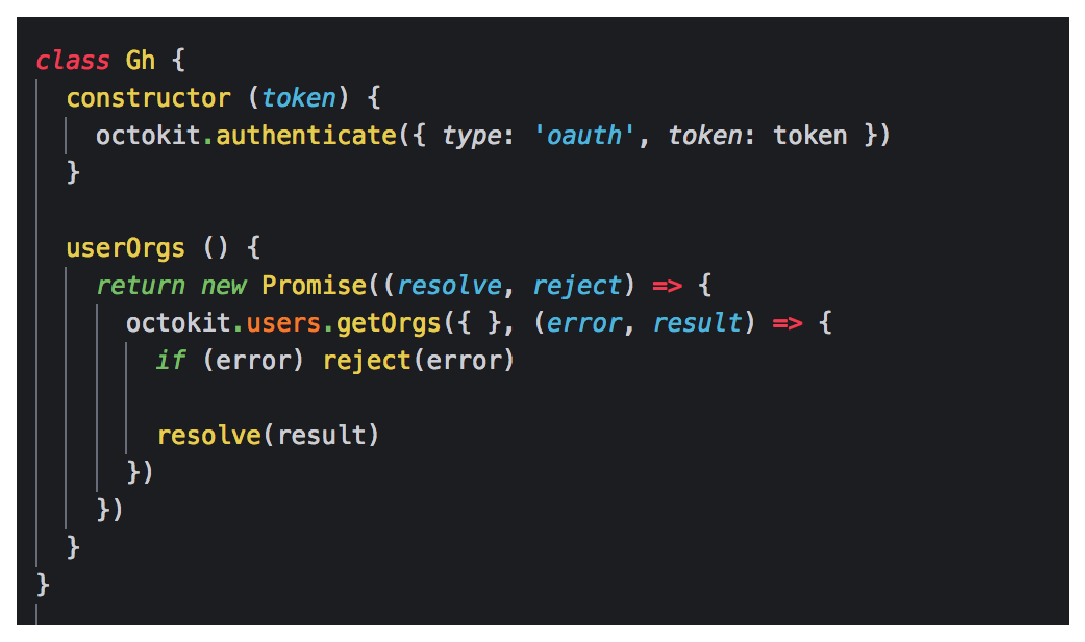
\includegraphics[scale=0.5]{images/clasegh}
\caption{Clase Github}
\label{fig:Clase Github}
\end{center}
\end{figure}

Las funcionalidades que aporta la API a Codelab son las siguientes:

\begin{itemize}
  \item Oauth
  \item Obtener las organizaciones del usuario para usar .
  \item Añadir usuarios a la organización.
  \item Crear un repositorio en las organizaciones.
  \item Añadir colaboradores al repositorio.
  \item Crear equipos.
  \item Añadir un equipo a un repositorio.
  \item Comprobar si un usuario es miembro de un equipo.
  \item Obtener los repositorios de una organización.
  \item Crear un fichero en un repositorio.
\end{itemize}

%++++++++++++++++++++++++++++++++++++++++++++++++++++++++++++++++++++++++++++++
\section{Modelo-Vista-Controlador}
\label{:sec3}

\subsection{El MVC}
\label{3:3:1}

El modelo vista controlador es una arquitectura de software que separa la lógica de la aplicación de la interfaz de usuario. Lo hace separando la aplicación en tres partes: el modelo, la vista y el controlador.

El modelo maneja los datos fundamentales, responde a las solicitudes de información, solicitudes para insertar, actualizar o eliminar la información. Esto podría ser una base de datos o cualquier sistema de estructura de datos. En resumen, es la gestión de datos y datos de la aplicación.

La vista proporciona la interfaz de usuario de la aplicación. Transformará los datos del modelo para mostrarselos al usuario de forma que pueda entender y manejar la información de forma sencilla e intuitiva.

El controlador recibe los datos y acciones del usuario y realiza llamadas al modelo para manejar los datos y a la vista para mostrar el resultado de dichas acciones.

\begin{figure}[!th]
\begin{center}
\includegraphics[scale=0.3]{images/29}
\caption{MVC}
\label{fig:MVC}
\end{center}
\end{figure}

\subsection{MVC en Codelab}
\label{3:3:2}

En la plataforma Codelab se ha implementado el Modelo Vista Controlador,
usando las funciones que nos proporciona Express.JS.

En el caso de las vistas Express nos permite establecer un motor de vistas.

\begin{figure}[!th]
\begin{center}
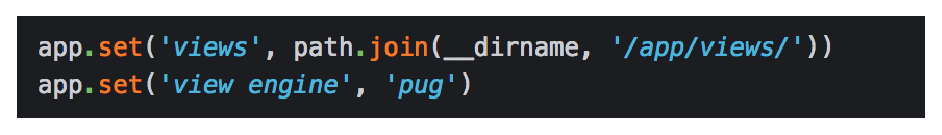
\includegraphics[scale=1.0]{images/defvistas}
\caption{Motor de vistas}
\label{fig:Motor de vistas}
\end{center}
\end{figure}

Con la primera línea de código le indicamos que la carpeta de vistas estará en el directorio app/views y con la segunda línea le indicamos que motor de vistas usaremos: Pug JS. 

En el código de abajo se puede ver la vista de error, que muestra al usuario el error y se le muestra el mensaje de error según el mensaje que se le pase desde el controlador.

\begin{figure}[!th]
\begin{center}
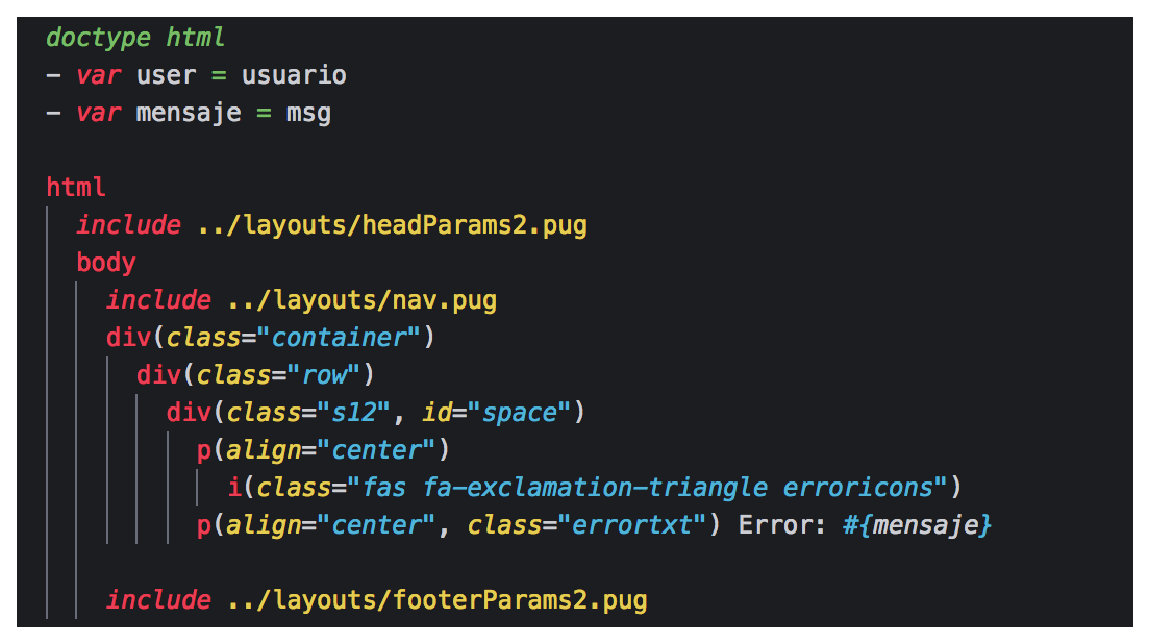
\includegraphics[scale=0.5]{images/vista}
\caption{Ejemplo de vista en Pug}
\label{fig:Ejemplo de vista en Pug}
\end{center}
\end{figure}

Pug es un motor de vistas bastante potente. Se pueden modular las vistas para reutilizar código y evitar repetirlo.
Por ejemplo, se puede dividir el código en Head donde se definen los distintos enlaces al CSS, JS y se pone el titulo, 
Nav que contiene la barra de navegación, que es igual para todos, el body que es el contenido de la vista y por último el footer.
También se pueden hacer bucles para mostrar las tareas o las aulas o mostrar un valor u otro dependiendo de si se tiene rol de alumno o de profesor.

\newpage

En el caso de los modelos se usa Mongoose y estarán ubicados en la carpeta de app/models. Los modelos le prorcionan la información a los controladores usando las funciones de mongoose, find, update, delete y save entre otras.

\begin{figure}[!th]
\begin{center}
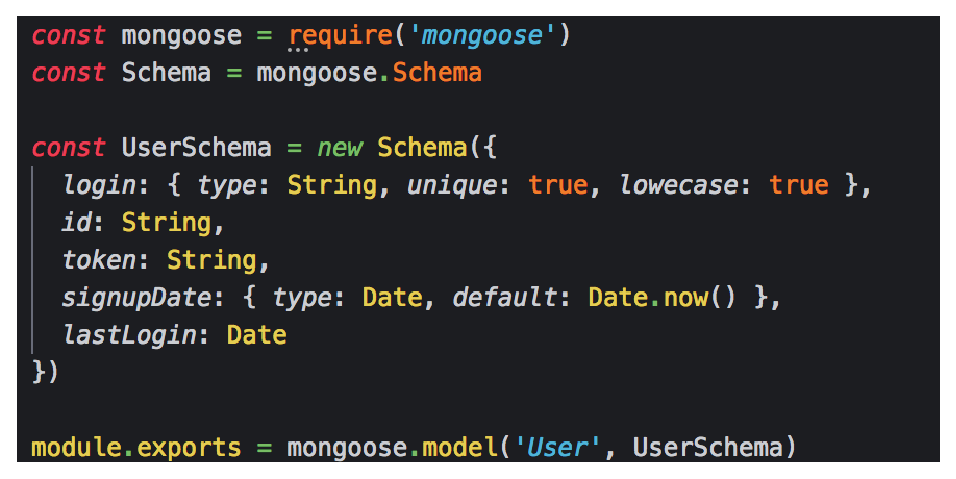
\includegraphics[scale=0.5]{images/modelo}
\caption{Ejemplo de modelo}
\label{fig:Ejemplo de modelo}
\end{center}
\end{figure}

Y por último, en el caso de los controladores, se definen funciones con las tareas que tienen que hacer
de forma que todo esta modulado. El controlador le pasa la información a las vistas usando el comando render, que renderiza la vista de Pug a HTML.


\begin{figure}[!th]
\begin{center}
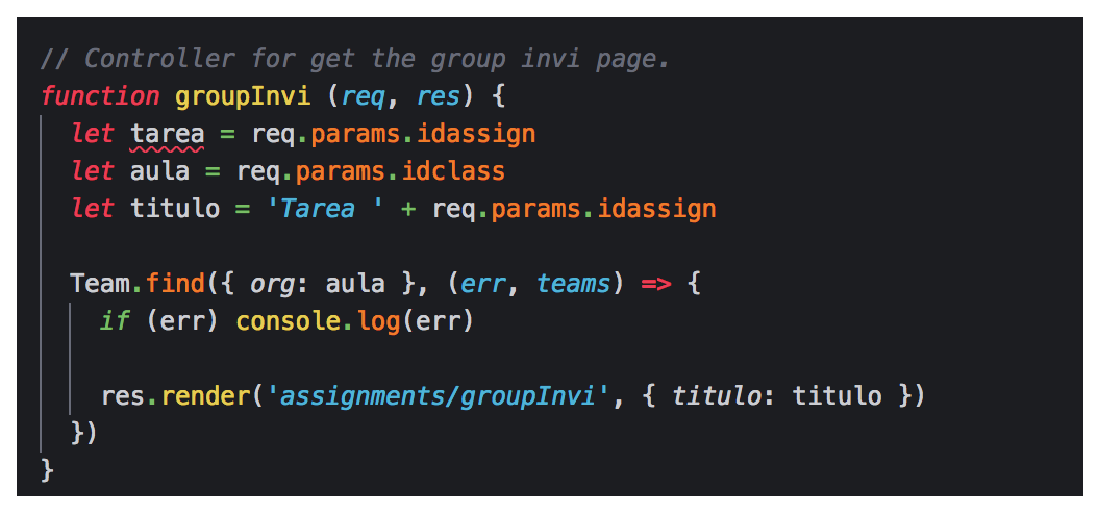
\includegraphics[scale=0.5]{images/controlador}
\caption{Ejemplo de Controlador}
\label{fig:Ejemplo de Controlador}
\end{center}
\end{figure}

Router se usa para crear rutas modulares. Una instancia Router es un sistema de middleware y direccionamiento completo que a menudo se denomina pequeña aplicación o miniapplicación.

Cabe destacar que para las rutas genéricas como aula o asignación en la que se puede representar los datos de cualquier aula o asignación se usan rutas que dependen de parámetos, es decir, rutas que muestran unos datos dependiendo de los parámetros que se le pasen.

\begin{figure}[!th]
\begin{center}
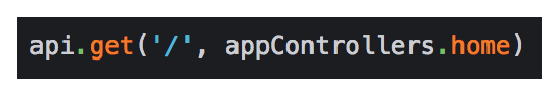
\includegraphics[scale=1.0]{images/ruta}
\caption{Ejemplo de ruta}
\label{fig:Ejemplo de ruta}
\end{center}
\end{figure}

%++++++++++++++++++++++++++++++++++++++++++++++++++++++++++++++++++++++++++++++

\section{Diseño de la base de datos}
\label{:sec4}

%++++++++++++++++++++++++++++++++++++++++++++++++++++++++++++++++++++++++++++++

\section{Funcionalidades para profesores}
\label{:sec5}

%++++++++++++++++++++++++++++++++++++++++++++++++++++++++++++++++++++++++++++++

\section{Funcionalidades para alumnos}
\label{:sec6}

%++++++++++++++++++++++++++++++++++++++++++++++++++++++++++++++++++++++++++++++

\section{Codelab vs Classroom}
\label{:sec7}

%++++++++++++++++++++++++++++++++++++++++++++++++++++++++++++++++++++++++++++++

\section{Metodología}
\label{:sec8}

%++++++++++++++++++++++++++++++++++++++++++++++++++++++++++++++++++++++++++++++